\chapter{基于网络拓扑的自动负载均衡策略}

在MoE(混合专家)训练模型中,专家的计算负载不均衡问题可能会对模型的训练效果产生影响。
% 
如果某些专家的计算负载过高,可能会导致模型训练变慢,甚至出现不收敛的情况。
% 
为了避免这种情况的发生,需要设计一种负载均衡算法来实现专家之间的计算负载均衡,实现较好的系统整体性能。

当设计负载均衡算法时,除了考虑专家的负载变化情况,还需要考虑训练系统的实际拓扑连接情况。不同的拓扑结构可能对负载均衡策略有不同的影响。
% 
在分布式拓扑中,不同的专家可能分布在多个节点上,通过网络进行通信。在这种情况下,负载均衡的策略需要考虑节点之间的通信开销和计算资源分配的平衡。

因此我们需要综合考虑专家负载、拓扑结构和通信开销之间的关系,选择合适的策略来实现负载均衡。这样可以提高训练系统的效率,减少通信开销,并加快模型的收敛速度。

\section{负载均衡算法概述}

\subsection{GPU集群网络拓扑结构}

Spine-leaf架构是一种常见的数据中心网络拓扑结构,用于构建高性能的GPU集群。它将数据中心网络划分为两个层级:Spine层和Leaf层。在该拓扑结构中,节点之间的通信是基于TCP/IP协议的以太网通信。

\begin{figure}[h!]
    \vskip 2ex
    \centering
    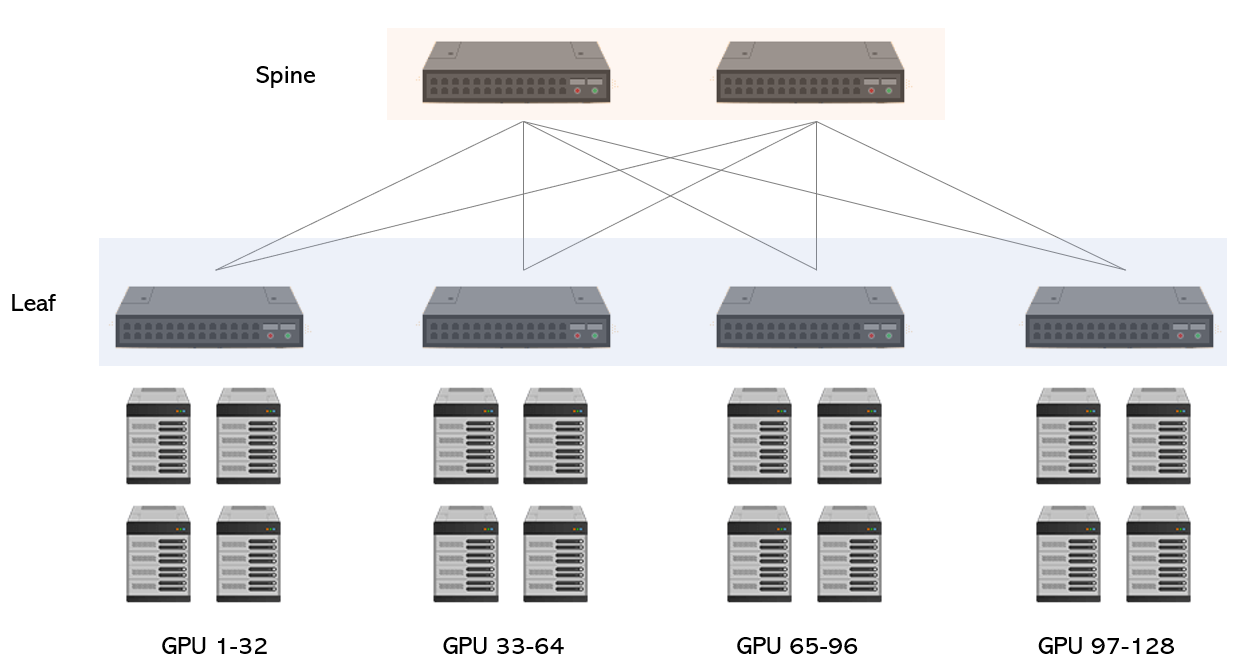
\includegraphics[width=0.7\linewidth]{figures/fig8.png}
    \caption{Spine-leaf GPU数据中心架构}
    \label{fig-GPU-ARCH}
    \end{figure}
    

Spine-leaf架构中,Spine层和Leaf层之间通过高速物理链路连接。每个Leaf节点连接多个GPU设备(一般为ToR交换机),而每个Spine节点则连接多个Leaf节点。通信过程中,数据包从源节点的GPU设备开始,通过本地的交换机和链路,经过目标节点的交换机,最后到达目标节点的GPU设备,以完成通信。

在Spine-leaf架构GPU拓扑结构中,通信可以分为两种类型:内部通信和外部通信。
\begin{itemize}
    \item \textbf{内部通信}:指的是同一台Leaf节点内部的GPU设备之间进行的通信(在同一机架内),这种通信只需要经过本地的交换机和链路即可完成。
    \item \textbf{外部通信}:是指不同Leaf节点之间的GPU设备之间进行的通信(跨机架GPU通信),这种通信需要经过Spine节点和目标Leaf节点的交换机和链路,这增加了传输的延迟和可能的网络拥塞。通常会采用高速的物理链路和交换机来连接Spine节点和Leaf节点,以提供相对较高的传输带宽以确保数据包能够到达目标GPU设备,但通信延迟和带宽可能相对较低。
\end{itemize} 

Spine-leaf架构GPU拓扑结构的优势在于提供了高性能、低延迟的通信,同时具有良好的可扩展性。该拓扑结构能够满足大规模GPU集群的通信需求,并支持高吞吐量的数据传输。通过合理设计和配置Spine-leaf架构,可以实现有效的负载均衡和网络流量管理,以提高GPU集群的整体性能和可靠性。

\subsection{GPU节点通信模型设计}

我们在GPU集群的架构上,使用了Alpha-Beta模型建立集群节点通信模型,Alpha-Beta模型是一种常见的建模方法,它可以有效地描述集群节点之间的通信行为,并为集群性能优化提供重要的参考依据。这样的建模方式,通过估计节点间通信成本,可以表示出任务的数据通信需求和节点的资源状况,从而优化任务调度和负载均衡策略,以提高整个集群的性能和效率。

\subsubsection{Alpha/Beta的含义}

\begin{itemize}
    \item \textbf{Alpha}: 表示数据包在发送过程中的传输时间,即数据包从发送节点到达接收节点的时间延迟。它可以涉及网络传输延迟、路由器处理时间、链路拥塞等因素。
    \item \textbf{Beta}: Beta表示数据包的传输带宽或吞吐量,即在单位时间内可以传输的数据量。它通常与网络带宽、链路容量以及节点处理能力相关。
\end{itemize}

\subsubsection{Alpha/Beta如何测量}


在建立集群节点通信模型时,可以使用Alpha-Beta模型来估计节点之间数据包发送的成本。这个成本可以通过以下因素进行建模:
通常我们可以连续发送k次大小为M的数据包,测量总共的发送时间${T_1}$,此时${T_1 = k * (alpha + \frac{M}{Beta})}$。
% 
之后发送一次大小为K*M的数据包,测量发送时间${T_2}$,这里的${T_2} = alpha + \frac{k * M}{Beta}$,之后联立以上两个方程,即可求解出任意两个节点的alpha/beta值。

此后任意两节点发送数据的大小即可使用求解出的alpha/beta进行表示。其中相同节点内的GPU之间具有较小的alpha/beta值,而节点之间的GPU传输具有较大的alpha/beta值。

\subsection{MoE训练系统专家负载变化情况}

在MoE训练中,每个子模型都是一个专家,需要处理一定比例的输入数据。不同的子模型可能具有不同的负载,即它们需要处理不同数量的输入数据。这是因为在MoE模型中,每个子模型负责处理不同类型的输入数据,因此在训练过程中,每个专家的负载可能会根据输入数据发生变化。

此外,同一专家的负载在不同时刻也会发生变化。这是因为在MoE训练中,子模型的权重和负载是动态调整的,以适应不同的输入数据分布和模型性能。因此,在训练过程中,同一专家的负载可能会根据模型的状态和数据的分布发生变化。


我们使用 Transformer-xl模型\ucite{dai2019transformer},将其原本的模型拓展为MoE架构,并对其第一层16个专家的负载情况做了统计。如图\ref{fig-transformer-xl}所示,我们发现随着时间的变化MoE模型的负载也随之变化,并不是静态不变的,有部分专家的负载甚至接近0,因此我们需要根据负载的变化情况,寻找最合适的策略。

为了解决MoE训练中的负载不均衡问题,可以采用一些负载均衡技术,例如动态调整权重、分配数据等,以确保每个子模型都能够得到足够的训练和优化。此外,还可以通过调整MoE模型的结构和参数来平衡不同专家之间的负载,以提高模型的训练效率和准确度。

总之,MoE训练中每一层之间的负载情况都不同,同时同一专家的负载再不同时刻也会发生变化。因此,在MoE模型的设计和训练过程中,需要考虑负载均衡问题,以提高模型的性能和准确度。

\subsection{负载均衡算法设计}

基于以上三点考虑,我们设计了一种基于网络拓扑的自动负载均衡策略,我们将MoE训练中涉及到的All-to-All通信过程建立成alpha-beta数学模型。由于MoE模型训练中通信是主要的开销,因此我们将训练的问题建模为组合优化问题,通过求解器求解基于当前负载情况的最合适的负载均衡策略。

我们对MoE模型训练的每一层都建立有一个优化问题。下面以一层为例,介绍优化模型的主要内容。优化模型的目标函数为全局节点之间的All-to-All成本最小。

\subsubsection{优化问题的输入数据}

优化模型的主要输入信息为:

\begin{enumerate}
    \item 专家总数为 $E$

    \item 设备总数为 $P$
    
    \item 一张GPU上一个MoE层最多可以放置的专家数目为 $L$
    
    \item 节点i与节点z之间的建立的网络模型的alpha值 $\alpha_{ij}$,用于表示任意两点网络连接的时间
    
    \item 节点i与节点z之间网络带宽的beta值 $\beta_{ij}$,表示网络传输速率;
    
    \item 当前系统每个专家的负载情况,即可表示为GPU $i$ 到专家 $e$ 总发送数据比例$C_{i,e}$
\end{enumerate}

\subsubsection{优化问题的求解参数}

优化问题的求解参数主要是每张GPU上可以放置哪些expert,以及每张GPU上原本拥有的数据需要发送到对应目标GPU上的比例,用字母表示出来分别是:
\begin{enumerate}
    \item 放置矩阵 $R$,表示每个专家应该放置在哪些 GPU 上。其大小为 $P \times E$,表示有 $P$ 个设备和 $E$ 个专家。
    $$R \in \mathbb{Z}^{P \times E}$$

    \item 发送数据矩阵 $W$,表示数据从一个 GPU 到另一个 GPU 的比例。其大小为 $P \times P \times E$,表示有 $P$ 个设备,每个设备发送数据到其他 $P-1$ 个设备中的 $E$ 个专家。
    $$W \in \mathbb{R^{+}}^{P \times P \times E}$$
\end{enumerate}

\subsubsection{优化问题的约束条件}

\begin{enumerate}

    \item  每个 GPU 上放置的专家数量不超过 $L$:
$$\sum_{k=1}^{E} R_{j,k} \leq L, \quad \forall j=1,2,\ldots,P$$
其中 $\sum_{k=1}^{E} R_{j,k} \leq L$ 表示对矩阵 $R$ 按行求和不能超过2。

\item 每种类型的专家必须存在:
% $$\min[\operatorname{SUM}(R, \text{dim}=0)] \geq 1$$
$$\sum_{j=1}^{P} R_{j,k} \geq 1, \quad \forall k=1,2,\ldots,E$$

其中 $R_{j,k}$ 表示专家 $k$ 是否被放置在 GPU $j$ 上,其取值为 $0$ 或 $1$。每种专家 $k$ 必须至少被一个 GPU 放置,即 $\sum_{j=1}^{P} R_{j,k} \geq 1$,应该对所有的专家 $k$ 进行约束。

\item 数据发送比例的和为 $1$:
$$\sum_k W_{i,j,k} = 1$$

其中 $W_{i,j,k}$ 表示从 GPU $i$ 发送到 GPU $j$ 的数据比例中,专家 $k$ 所占的比例。

\item 当不存在专家时,数据发送比例必须为 $0$:
$$R_{j,k} = 0 \Rightarrow W_{i,j,k} = 0$$

其中 $R_{j,k}$ 表示专家 $k$放置在 GPU $j$ 上,$W_{i,j,k}$ 表示从 GPU $i$ 发送到 GPU $j$ 的数据比例中,专家 $k$ 所占的比例。
\end{enumerate}

\subsubsection{优化问题目标函数}



$$  \operatorname{MIN} \left( \sum_i \sum_j \left( a_{i,j} + \frac{V_{i,j}}{b_{i,j}} \right) \right)$$

其中 $\operatorname{MIN}$ 表示对所有可能的解求最小值,$a_{i,j}$ 表示建立从 GPU $i$ 到 GPU $j$ 的网络连接需要的时间,$b_{i,j}$ 表示从 GPU $i$ 到 GPU $j$ 的网络传输速率的倒数,$V_{i,j}$ 表示从 GPU $i$ 发送到 GPU $j$ 的数据量,其计算如下:

$$V_{i,j} = \sum_{k=1}^{E} R_{j,k} \cdot W_{i,j,k} \cdot C_{i,k} \cdot \left(1-R_{i,k}\right)$$

$R_{j,k}$ 表示专家 $k$ 是否被放置在 GPU $j$ 上,$W_{i,j,k}$ 表示从 GPU $i$ 发送到 GPU $j$ 的数据比例中,专家 $k$ 所占的比例,$C_{i,k}$ 表示从 GPU $i$ 发送到专家 $k$ 的数据量。该式表示在数据从 GPU $i$ 发送到 GPU $j$ 的过程中,需要发送所有的数据量。

\section{负载均衡算法系统实现}

我们在已有的MoE训练框架上进行了相关改进,我们主要采用了Deepspeed-MoE训练框架。
% 
DeepSpeed-MoE\ucite{rajbhandari2022deepspeed}是一种基于 DeepSpeed 分布式深度学习框架的 Mixture of Experts (MoE) 模型实现,它为用户提供了一个可扩展且高性能的MoE训练框架。通过在Deepspeed的源码上做出修改,我们可以实现高性能和高效的分布式训练解决方案。
% 
具体而言,我们在Deepspeed框架的基础上实现了负载均衡算法。对原本的DeepSpeed-MoE分布式深度学习框架训练过程中对系统的负载进行优化和均衡。
% 
Deepspeed也是我们训练系统在性能比较时的一个baseline。


\subsection{系统实现}

\begin{enumerate}
    \item 专家并行初始化:我们引入了专家-数据并行组(expert-data-parallel-group)的概念。这个组的建立旨在实现对专家和数据的并行处理。通过这一修改,我们能够同时在不同设备上进行专家和数据的计算,从而提高训练速度和效率。
    \item 训练阶段1:我们移除了可以在本地计算的All-to-All参数,并将其替换为全零。这个调整旨在减少通信开销,避免不必要的数据传输。在这一步中我们主要完成每个节点内部的GPU之间相互交换数据。
    \item 训练阶段2:在第二轮训练开始时,我们进行本地计算。这意味着一部分计算可以在每个设备上独立完成,并进行全局的GPU数据交换,这意味着,我们可以将计算过程与通信重叠,并进一步提高训练的速度和效率。
    \item 训练阶段3:在每轮训练的结束时,使用reduce原语计算负载跟踪(load trace)。这一修改有助于监控每个设备的负载情况,从而了解训练过程中的负载分布。
    \item 训在训练结束时,我们将MoE参数通过All-Reduce操作同步。这一步骤确保了MoE参数的正确同步,以获得准确的模型结果。通过正确的同步,我们可以确保模型的一致性和准确性。
    \item 达到设定迭代轮次:在达到指定步骤后,我们引入了Gurobi优化算法,用于计算负载均衡策略。这一修改允许我们在特定轮次后通过优化算法调整专家的放置位置,以进一步优化模型的性能。通过优化放置策略,我们可以更好地利用集群资源,提高训练效率和模型性能。
    \item 更新专家放置以适应当前负载:在达到指定步骤后,我们进行专家参数的交换。这一修改涉及在不同设备之间传输和同步专家参数,以更好地利用各设备的计算资源。通过根据当前负载情况调整专家的放置位置,我们可以实现负载的动态均衡,进一步提高训练的效率和性能。
    \item 重复迭代直到模型收敛。我们的负载均衡算法系统会在模型收敛之前反复执行上述步骤,以确保模型能够充分训练和收敛。通过迭代的过程,我们能够不断优化负载均衡策略,提高系统的整体性能和训练效果。

\end{enumerate}

在训练的过程中,我们还设计了一个scheduler用于监控并收集专家的负载情况,该调度器是负载均衡算法系统中的关键组件,通过定期收集和分析专家的负载信息,能够及时地检测到系统中的负载变化。它会综合考虑整个集群中各个专家的负载状态,识别出负载较重或负载较轻的专家,并根据负载不均衡的程度进行优化调度。

通过以上一系列的定制修改,我们对DeepSpeed框架进行了个性化的定制,以满足特定需求。这些调整的目标在于提高训练速度、优化资源利用、调整专家的放置策略,并确保模型参数的正确同步。这些改进对于MoE模型的训练过程具有重要意义,有望提升性能和效果。

\section{本章小结}

总结起来,通过我们对DeepSpeed框架的修改和补充,以及对MoE训练过程的优化,我们能够实现负载均衡算法系统,监控和调度专家的负载情况,从而提高训练效率和模型性能。这些改进措施包括并行化处理、减少通信开销、本地计算、负载跟踪、参数同步、放置策略优化和专家参数交换等。通过持续迭代和优化,我们能够达到更好的负载均衡效果,并在训练过程中实现模型的收敛。这些改进为深度学习任务的分布式训练提供了更好的性能和效果,为研究者和工程师提供了有力的工具和方法。

\endinput